%/// @file   Report.tex
%/// @author Markovich Dmitry <dmmrkovich at gmail (.) com>
%/// @copyright 2013 Markovich Dmitry
%/// @section LICENSE
%/// GNU General Public License.

\documentclass[10pt]{article}
\usepackage[T2A]{fontenc}
\usepackage[utf8]{inputenc}
\usepackage[russian,english]{babel}
\usepackage{amssymb,amsmath}
\usepackage{graphicx}
%\usepackage{abstract}
\graphicspath{{images/}}
\author{Д. Маркович,~К. Ладутенко,~П. Белов}

\title{Поиск оптимальной реализации метода FDTD}
\date{\today}
\begin{document}
\maketitle
% \address{Санкт-Петербургский Национальный Исследовательский Университет 
%   Информационных технологий, Механики и Оптики (НИУ ИТМО), 
%   Санкт-Петербург, Россия}
\renewcommand{\abstractname}{}
%\renewcommand{\absnamepos}{empty}
\begin{abstract}
  В этом тексте приводится сравнение быстродействия реализаций
  метода конечных временных разностей (finite-difference time-domain
  method, FDTD) с помощью Fortran, С и C++ (с использованием
  библиотеки Blitz++) для разных аппаратных платформ (AMD, Intel i5,
  Intel Xeon). Кратко описываются особенности каждой из 
  перечисленных реализаций, для заданных параметров вычислительной задачи 
  указывается наиболее эффективная из них. + НЕКИЙ ВЫВОД
\end{abstract}
\renewcommand{\contentsname}{Содержание}
%\tableofcontents{}
\section{Краткое описание метода FDTD}
\label{fdtd_basics}
Метод FDTD был предложен Кейном Йи в 1966 г. в оригинальной статье\cite{Yee1966},
однако название и аббревиатуру он получил от Аллена Тафлова, который сегодня 
считается одним из пионеров теории и практики метода\cite{Taflove}. По сути
FDTD представляет собой сеточный метод решения уравнений Максвелла в 
дифференциальной форме. В общем случае эти уравнения имеют вид:
\begin{eqnarray}
rot~\bf E = -\mu\frac{\partial~\bf H}{\partial t} - \sigma_m~\bf H\\
rot~\bf H = \epsilon\frac{\partial~\bf E}{\partial t} + \sigma~\bf E
\end{eqnarray}
Вводя прямоугольную сетку и пространственные коэффициенты связи полей
\cite{udfdtd}, уравнения можно привести к алгоритму, позволяющему рассчитать
значения компонентов полей в "следующий" момент времени $t+1$ в заданной
точке пространства, если известны их значения в "предыдущий" момент времени $t$:
% \begin{eqnarray}
% H_{x,~t~+~1}^{m, n} = C_{H_xH,~t}^{m, n} \cdot H_{x,~t}^{m, n} -
% C_{H_xE,~t}^{m, n} \cdot \left( E_{z,~t}^{m, n + 1} - E_{z,~t}^{m, n}\right)\nonumber\\
% H_{y,~t~+~1}^{m, n} = C_{H_yH,~t}^{m, n} \cdot H_{y,~t}^{m, n} +
% C_{H_yE,~t}^{m, n} \cdot \left(E_{z,~t}^{m + 1, n} - E_{z,~t}^{m, n}\right)\nonumber\\
% E_{z,~t~+~1}^{m, n} = C_{E_zE,~t}^{m, n} \cdot E_{z,~t}^{m, n} +
% C_{E_zH,~t}^{m, n} \cdot \left(\left(H_{y,~t}^{m, n} - H_{y,~t}^{m - 1, n}\right) -
%  \left(H_{x,~t}^{m, n} - H_{x,~t}^{m, n - 1}\right)\right)\nonumber
% \end{eqnarray}
- для 2D случая и
% \begin{eqnarray}
% H_{x,~t~+~1}^{m, n, p} = C_{H_xH,~t}^{m, n, p} \cdot H_{x,~t}^{m, n, p} +
% C_{H_xE,~t}^{m, n, p} \cdot \left(\left(E_{y,~t}^{m, n, p + 1} -
% E_{y,~t}^{m, n, p}\right) -\left(E_{z,~t}^{m, n + 1, p} - E_{z,~t}^{m, n, p}\right)
% \right)\nonumber\\
% H_{y,~t~+~1}^{m, n, p} = C_{H_yH,~t}^{m, n, p} \cdot H_{y,~t}^{m, n, p} +
% C_{H_yE,~t}^{m, n, p}\cdot\left(\left(E_{z,~t}^{m + 1, n, p} - E_{z,~t}^{m, n, p}\right)-
% \left(E_{x,~t}^{m, n, p + 1} - E_{x,~t}^{m, n, p}\right)\right)\nonumber\\
% H_{z,~t~+~1}^{m, n, p} = C_{H_zH,~t}^{m, n, p} \cdot H_{z,~t}^{m, n, p} +
% C_{H_zE,~t}^{m, n, p}\cdot\left(\left(E_{x,~t}^{m, n + 1, p} - E_{x,~t}^{m, n, p}\right)-
% \left(E_{y,~t}^{m + 1, n, p} - E_{y,~t}^{m, n, p}\right)\right)\nonumber\\
% E_{x,~t~+~1}^{m, n, p} = C_{E_xE,~t}^{m, n, p}\cdot E_{x,~t}^{m, n, p} +
% C_{E_xH,~t}^{m, n, p}\cdot\left(\left(H_{z,~t}^{m, n, p} - H_{z,~t}^{m, n - 1, p}\right)-
% \left(H_{y,~t}^{m, n, p} - H_{y,~t}^{m, n, p - 1}\right)\right)\nonumber\\
% E_{y,~t~+~1}^{m, n, p} = C_{E_yE,~t}^{m, n, p} \cdot E_{y,~t}^{m, n, p} +
% C_{E_yH,~t}^{m, n, p}\cdot\left(\left(H_{x,~t}^{m, n, p} - H_{x,~t}^{m, n, p - 1}\right)-
% \left(H_{z,~t}^{m, n, p} - H_{z,~t}^{m - 1, n, p}\right)\right)\nonumber\\
% E_{z,~t~+~1}^{m, n, p} = C_{E_zE,~t}^{m, n, p} \cdot E_{z,~t}^{m, n, p} +
% C_{E_zH,~t}^{m, n, p}\cdot\left(\left(H_{y,~t}^{m, n, p} - H_{y,~t}^{m - 1, n, p}\right)-
% \left(H_{x,~t}^{m, n, p} - H_{x,~t}^{m, n - 1, p}\right)\right)\nonumber
% \end{eqnarray}
для 3D случая. На практике более интересен 3D случай, однако в ряде задач
работает и 2D случай, поэтому он не выбрасывается из рассмотрения.
\section{Способы реализации метода FDTD}
\label{fdtd_coding}
На практике возникает вопрос оптимальной реализации метода FDTD, а именно
использование какого из языков программирования позволяет в однопоточном
режиме просчитать задачу с заданными параметрами быстрее всего. С момента 
своего появления (2-я половина 1950-х) и до начала 1990-х годов наиболее 
эффективным языком для научных и инженерных вычислений было принято считать 
Fortran, специально для этих целей и разработанный. Достаточно сказать, что в 
те времена программы, реализованные на Fortran были быстрее аналогов на C++ 
вплоть до десятка раз\cite{Todd1997}. Таким образом, нередко вычислительная 
часть программ писалась на Fortran, а возможности C++, такие как перегрузка 
операторов а также объектно-ориентированное и шаблонное программирование 
использовались для всех остальных целей. Ещё одним весомым плюсом Fortran 
несомненно можно считать наличие огромного количества свободно распространяющихся
библиотек. Тем не менее, улучшение оптимизации программного кода компиляторами 
C++ а также использование шаблонного программирования позволили ему уже во второй
половине 1990-х годов сравняться с Fortran по производительности. В данной работе
будет рассмотрена библиотека Blitz++\cite{blitz_web}, разработанная Тоддом
Вельдхузеном в 1997 году. Эта библиотека использует технику шаблонного
метапрограммирования на C++, оптимизируя математические операции с данными и
сохраняя при этом традиционный синтаксис (схожий с такими аналогами, как 
Fortran или Matlab), значительно ускоряя вычислительную часть программы по 
сравнению со стандартной реализацией C++.\\*
Т.к. цель данной работы заключается в нахождении оптимальной реализации
метода FDTD,то было решено проверить 3 способа : 1) Стандартный С++ 2) Fortran 
3) Blitz++
\subsection{Реализация на C++}
Типичная реализация метода FDTD на C++ выглядит следующим образом
(показан фрагмент функции для подсчёта поля $H_x$ в "следующий"
момент времени $t+1$ в 2D случае):\\*
\begin{verbatim}
for (int i = x1; i <= x2; ++i) {
  for (int j = y1; j <= y2; ++j) {
    data[1][kHx][i][j] = data[0][kChxh][i][j] *
      data[0][kHx][i][j] - data[0][kChxe][i][j] *
      (data[0][kEz][i][j + 1] - data[0][kEz][i][j]);
  }
}
\end{verbatim}
Реализация математических операций $+,-,\cdot,/$ в стандартном C++ крайне
неэффективна. Например, чтобы выполнить операцию $x=x_1+x_2+x_3$ необходимо
сначала подсчитать временный результат сложения $t_1=x_1+x_2,$ затем 
$t_2=t_1+x_3,$ и наконец присвоить $x=t_2$. В процессе вычисления все временные
результаты хранятся в памяти компьютера. Поэтому при выполнении математических
операций над массивами, особенно небольшой длины, когда на сохранение временных
данных тратится значительно больше времени, чем непосредственно на сами 
вычисления, С++ показывает низкую производительность.\\*
Количественную оценку времени счёта задачи с заданными параметрами
(количество шагов по времени и пространственный размер) можно получить,
замеряя время выполнения соответственно 2D или 3D алгоритма для метода FDTD. При
этом удобно ввести параметры $max\_size$ и $max\_steps$ и зафиксировать "общий" 
размер задачи $\left(C_{2D} = max\_size^2 \cdot max\_steps,C_{3D} = max\_size^3 
\cdot max\_steps \right),$ а затем изменять параметры, сохраняя значение $C.$
Также, следует нормировать время выполнения алгоритма на значение $C,$ получая
таким образом время счёта на узел сетки.
Следует отметить, что приведённые результаты получены с использованием флагов
оптимизации $-O2~-ftemplate-depth-30$ компилятора $gcc~4.4,$ что несомненно 
ускоряет счёт, однако, как станет ясно из дальнейшего, времена выполнения 
всё равно остаются слишком большими.
\subsection{Реализация на Fortran}
Реализация вычислительного алгоритма на Fortran 90/95 имеет более компактный
вид по сравнению с C++ благодаря встроенной возможности работать с частями
массива:\\*
\begin{verbatim}
data(1:size,1:size,Hx,1) = data(1:size,1:size,Chxh,0) * 
                            data(1:size,1:size,Hx,0) -
                             data(1:size,1:size,Chxe,0) *
                              (data(1:size,2:(size+1),Ez,0) -
                              data(1:size,1:size,Ez,0))
\end{verbatim}
Серьёзным отличием от приведённого выше фрагмента кода на C++ следует считать 
"неправильный" (с точки зрения C++) порядок расположения данных в памяти.
Например, элементы матрицы в Fortran располагаются не построчно, как в C++,
а постолбцово, а потому и эффективный алгоритм должен иметь отличающийся вид.
Результаты измерений времени выполнения алгоритмов на Fortran
с оптимизирующим флагом компиляции $-O2$ компилятора $gfortran~4.4$ представлены
Как можно видеть, Fortran действительно в разы быстрее C++.
Помимо уже упомянутых выше причин этому также способствует хорошая
оптимизация компилятором Fortran программного кода.
\subsection{Реализация на C++ с  Blitz++}
Реализация метода FDTD на C++ с использованием библиотеки Blitz++
(в дальнейшем просто "на Blitz++" для краткости) представляет особый интерес.
Как уже упоминалось выше, эта библиотека решает большинство проблем с
быстродействием C++ при помощи шаблонного метапрограммирования. Ускорение
достигается за счёт того, что перегруженные математические операторы 
$+,-,\cdot,/$ не возвращают промежуточные значения при вычислениях, и операции
выполняются значительно быстрее. Естественно, частично ускорение уменьшается 
из-за затрат времени на более сложный код, однако этот недостаток устраним при 
хорошей оптимизации компилятора C++. Также важно отметить наличие в библиотеке 
так называемой кэш-оптимизации. У современных процессоров имеется до трёх
уровней кэша, т.е. промежуточного буфера, доступ к данным которого 
осуществляется быстрее чем к данным в оперативной памяти. 1-й уровень кэша 
является наименьшим по объёму, зато быстрейшим по скорости доступа, 2-й уровень
кэша больше 1-го по объёму и медленнее по скорости доступа и т.д. При реализации
алгоритмов, как в методе FDTD, правильное расположение данных в памяти 
позволяет значительно увеличить частоту попадания данных в кэш, а следовательно
ускорить вычислительную часть программы. Кэш~-~оптимизация Blitz++ основана не
на методе разбиения массива на блоки, а на кривой Гильберта: код, при помощи 
техники шаблонного программирования, специальным образом преобразуется для
максимальной частоты попадания данных в кэш в независимости от используемой
платформы.\\*
Реализовать алгоритм метода FDTD в Blitz++ позволяют две операции над массивами:
$Range$ и $Stencil$. Первая генерирует диапазон целых чисел, в котором меняется
произвольный индекс массива, а затем выполняет действия над всеми элементами,
указанными в диапазоне. Аналогичный приведённым выше фрагмент кода имеет вид:\\*
\begin{verbatim}
const blitz::Range i(1, length_x);
const blitz::Range j(1, length_y);
data(1)(kHx, i, j) = data(0)(kChxh, i, j) * data(0)(kHx, i, j) -
                     data(0)(kChxe, i, j) *
                     (data(0)(kEz, i, j+1) - data(0)(kEz, i, j));
\end{verbatim}
$Stencil$ является более сложной операцией, не использующей явный вид 
индексации. Вместо этого $Stencil$ сама определяет диапазон изменения индексов,
основанный на размерах переданных ей в качестве аргумента массивов. 
Определённое неудобство доставляет невозможность работы с массивами размерности
более 3, однако его можно обойти. Фрагмент кода с этой операцией имеет вид:\\*
\begin{verbatim}
BZ_DECLARE_STENCIL5(update_field_Hx, kHx_next, kHx, kChxh, kChxe,
                                                             kEz)
kHx_next = kChxh * kHx - kChxe * (kEz(0, 1) - kEz);
BZ_END_STENCIL_WITH_SHAPE(blitz::shape(0, 0), blitz::shape(0, 1))
 
 applyStencil(update_field_Hx(), kHx_next, kHx, kChxh, kChxe,
                                                        kEz);
\end{verbatim}
\newpage
\section{Сравнение быстродействия приведённых реализаций}
Сравнения времён выполнения приведённых реализаций представлены ниже.
Времена счёта для Blitz++ уменьшились в разы по сравнению со стандартным C++,
и для большинства задач превосходят Fortran. Применение операции $Stencil$
даёт лучшие результаты для 2D алгоритма, а $Range~-$
для 3D (Рис.~\ref{2D_amd} и Рис.~\ref{3D_amd}).
\renewcommand{\figurename}{Рис.}
\begin{figure}[h]
\begin{minipage}[h]{0.99\textwidth}
\center{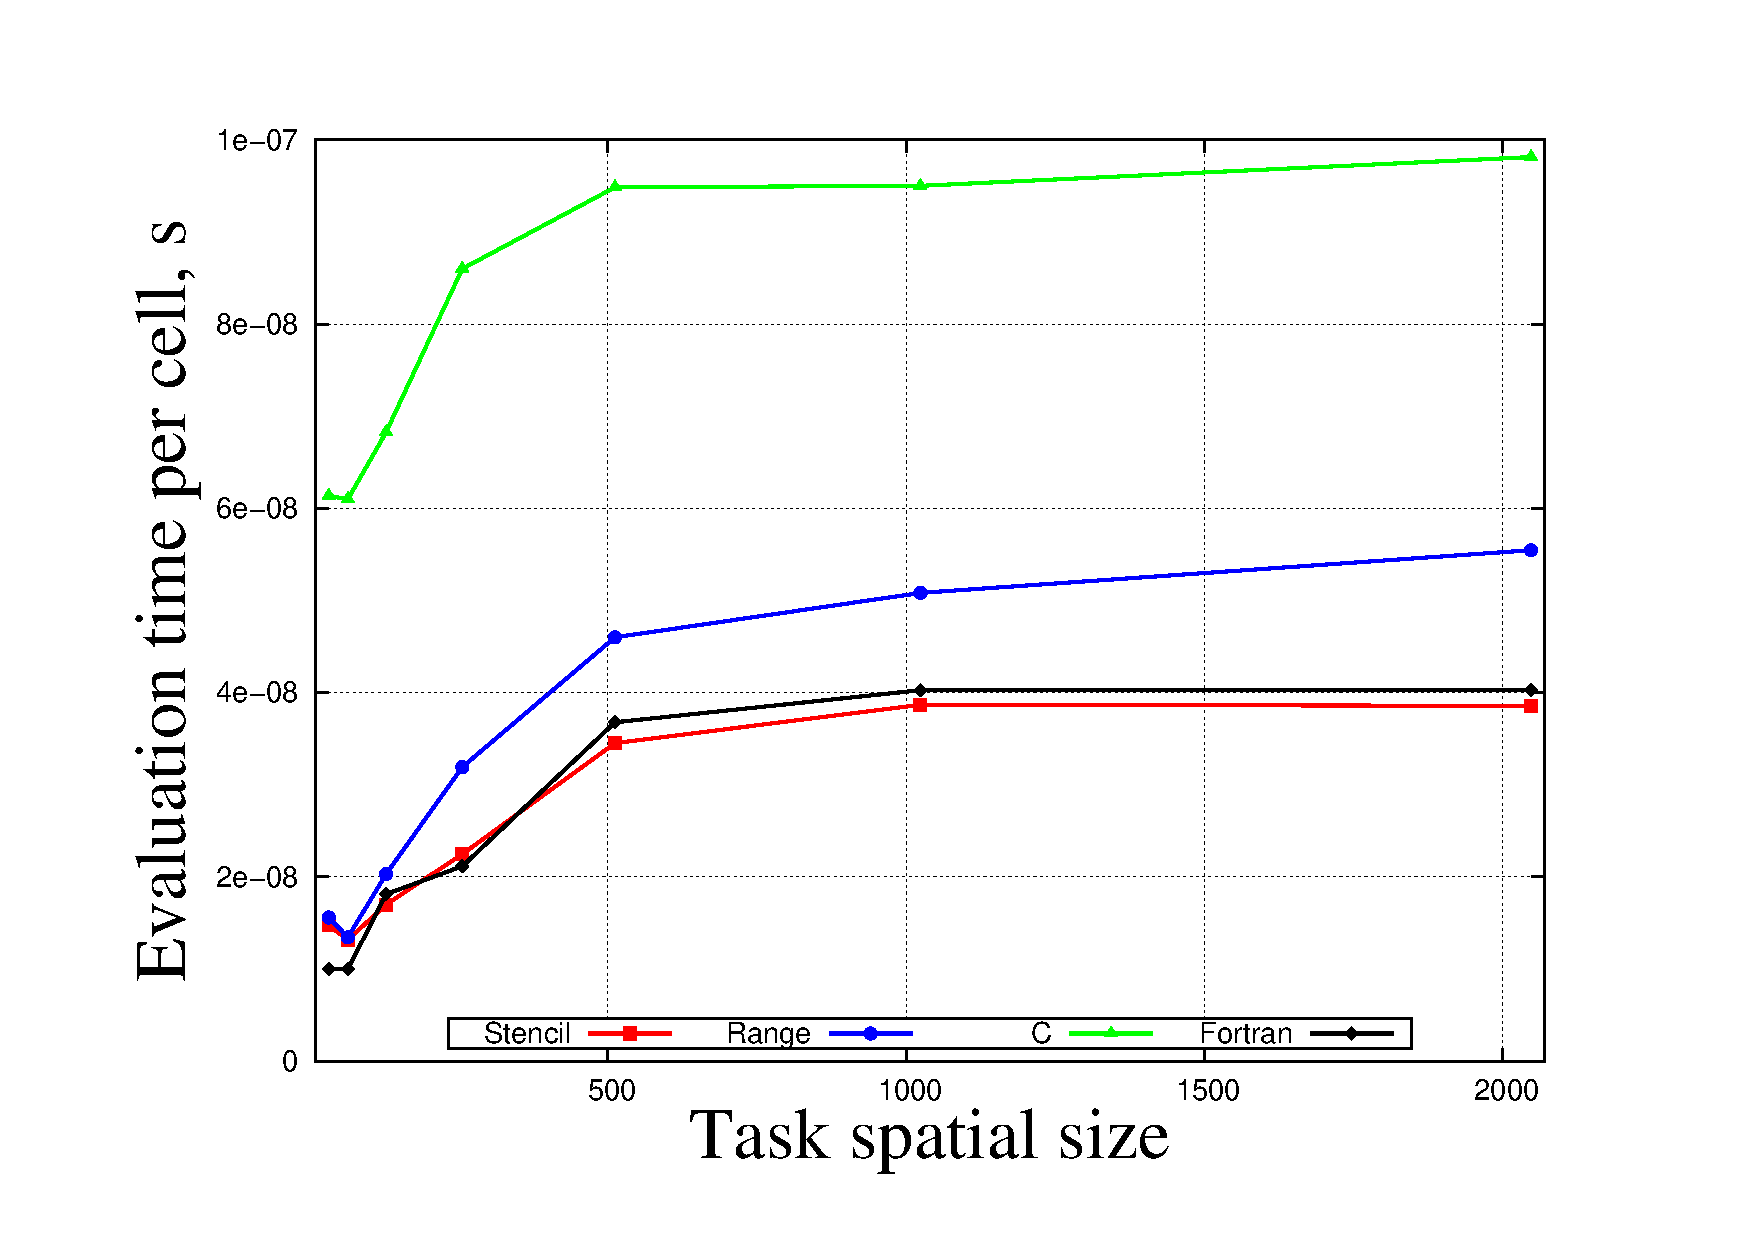
\includegraphics[width=0.7\textwidth]{2D_amd.pdf}}
\end{minipage}
\caption{Сравнение времён выполения 2D aлгоритма и в зависимости 
  от пространственного размера задачи для всех реализаций (AMD)}
\label{2D_amd}
\end{figure}
\begin{figure}[h]
\begin{minipage}[h]{0.99\textwidth}
\center{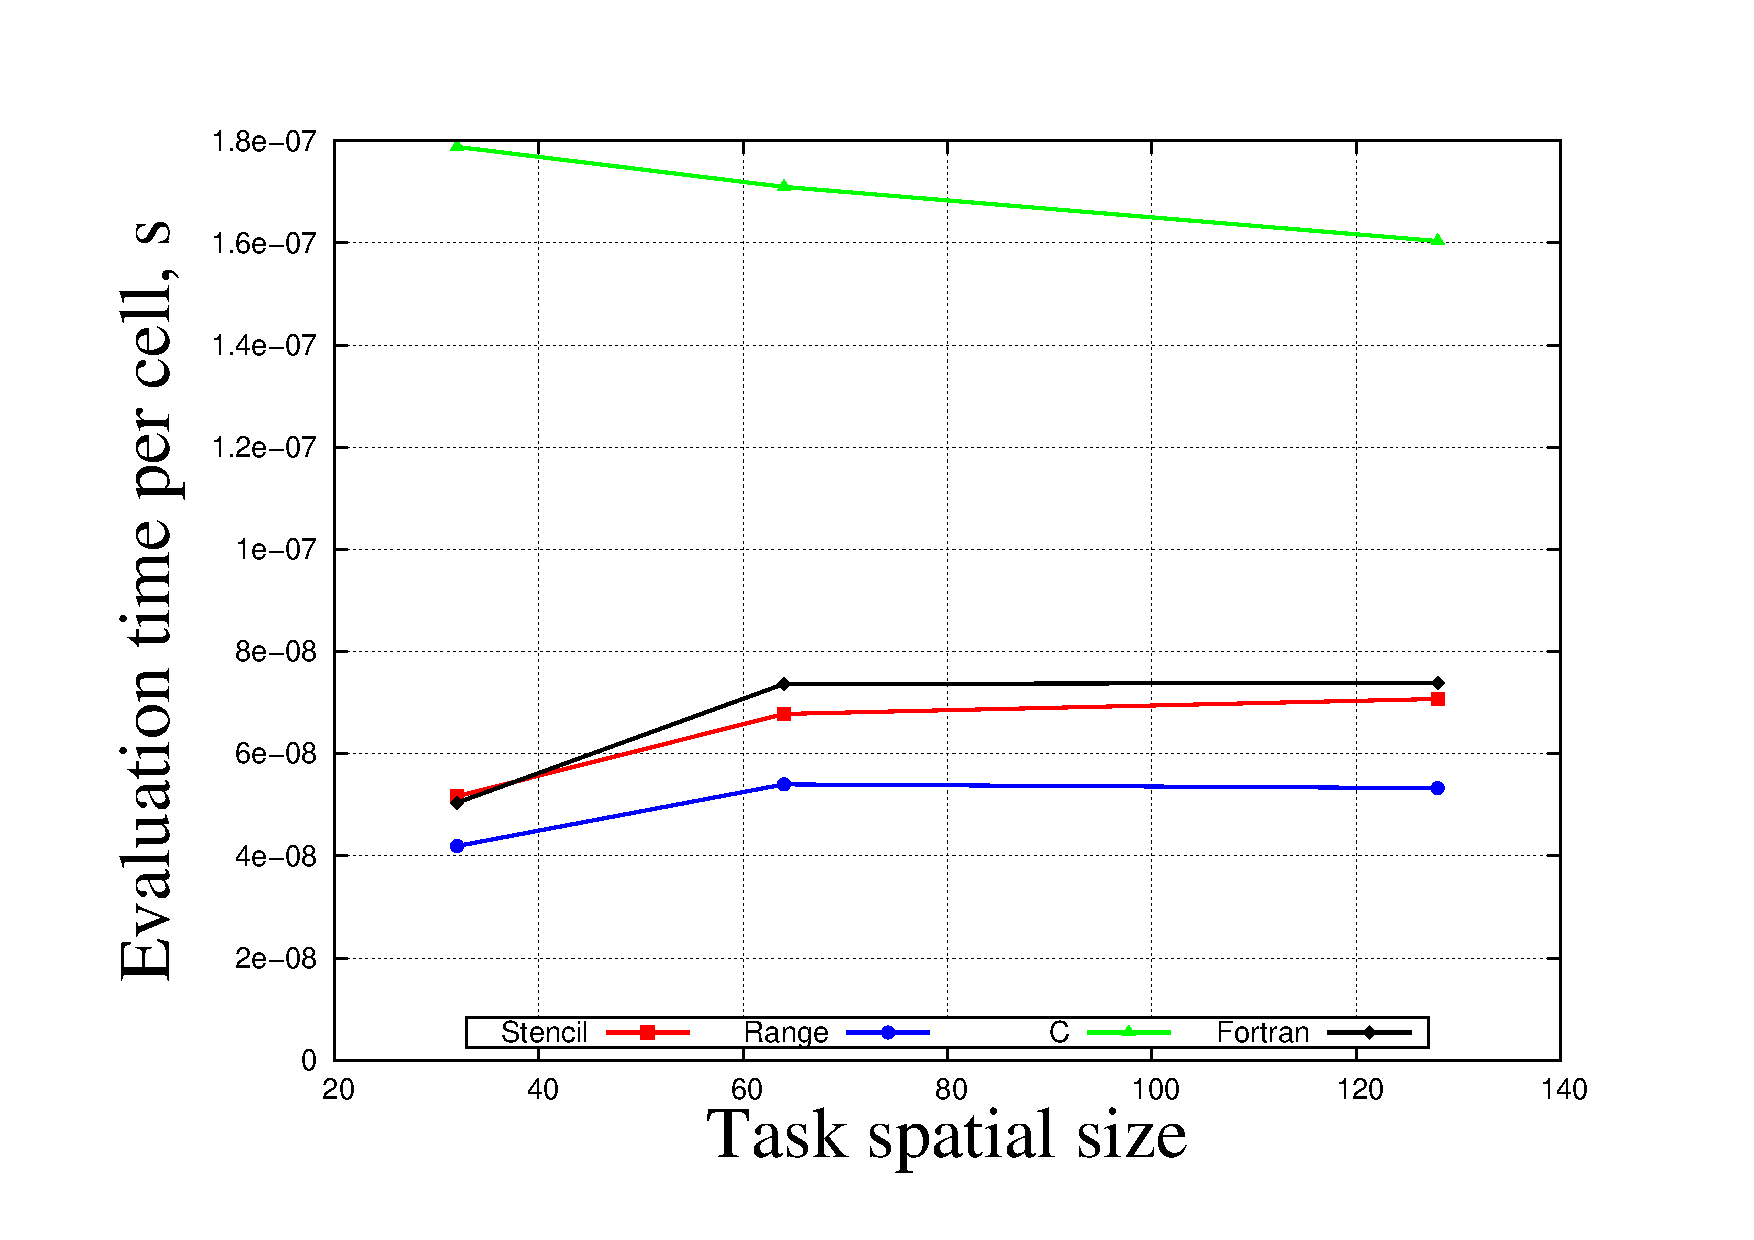
\includegraphics[width=0.7\textwidth]{3D_amd.pdf}}
\end{minipage}
\caption{Сравнение времён выполения 3D aлгоритма и в зависимости 
  от пространственного размера задачи для всех реализаций (AMD)}
\label{3D_amd}
\end{figure}
\clearpage
\section{Блочная оптимизация реализаций на Blitz++}
Однако, существует возможность дальнейшего увеличения
производительности за счёт дополнительных оптимизаций Blitz++ для некоторых
специальных размеров задачи. Например, можно применять операции $Range$ и 
$Stencil$ для рассчёта заданной области поблочно. Это позволит при правильном 
выборе размера блока для используемой платформы улучшить кэш-эффективность и 
получить дополнительное ускорение на размерах задачи, согласующихся с длиной
кэш-линии. Это предположение было проверено соответствующей дополнительной 
реализацией FDTD алгоритма с разбиением счётной области на блоки. Размер блока 
для каждой задачи менялся от минимальных 8 элементов, до половины размера самой 
задачи. Времена выполнения 2D алгоритма для реализаций с блоками в сравнении со 
"стандартными" реализациями $Range$ и 
$Stencil$ для задачи 1024 x 1024 представлены на графике (Рис.~\ref{1024_amd}).
\begin{figure}[h]
\begin{minipage}[h]{1\textwidth}
\center{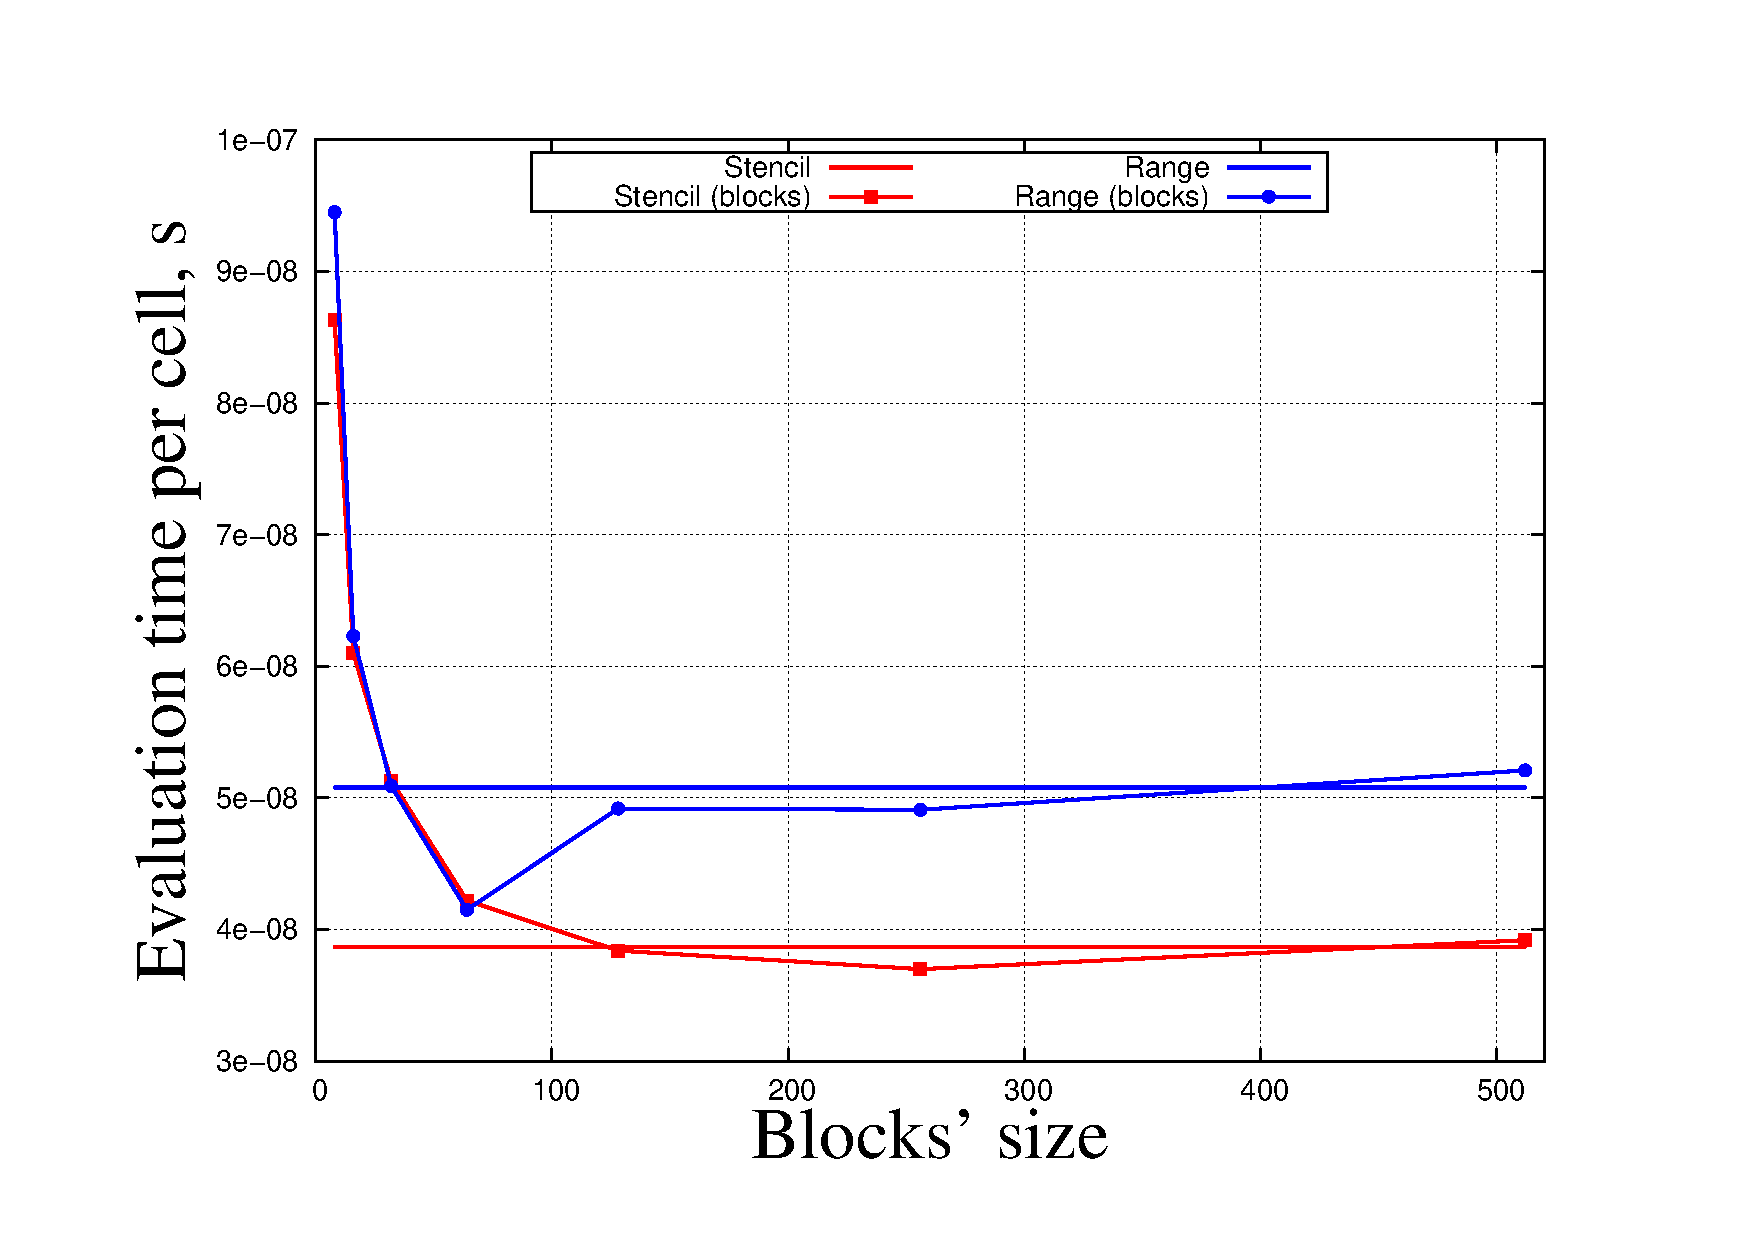
\includegraphics[width=1\textwidth]{1024_blocks_amd.pdf}}
\end{minipage}
\caption{Время выполнения 2D алгоритма с блоками для реализации на Blitz++ 
  для задачи 1024 x 1024 (AMD)}
\label{1024_amd}
\end{figure}
\clearpage
Для операции $Stencil$ 
наблюдается лишь незначительное улучшение, в то время как для $Range$ правильно
подобранный размер блока улучшает время выполнения вплоть до $\mathtt{\sim}$~20\%. В целом 
для всех исследуемых размеров сравнение реализаций показано на 
Рис.~\ref{2D_blocks_amd}.\\*
\begin{figure}[h]
\begin{minipage}[h]{1\textwidth}
\center{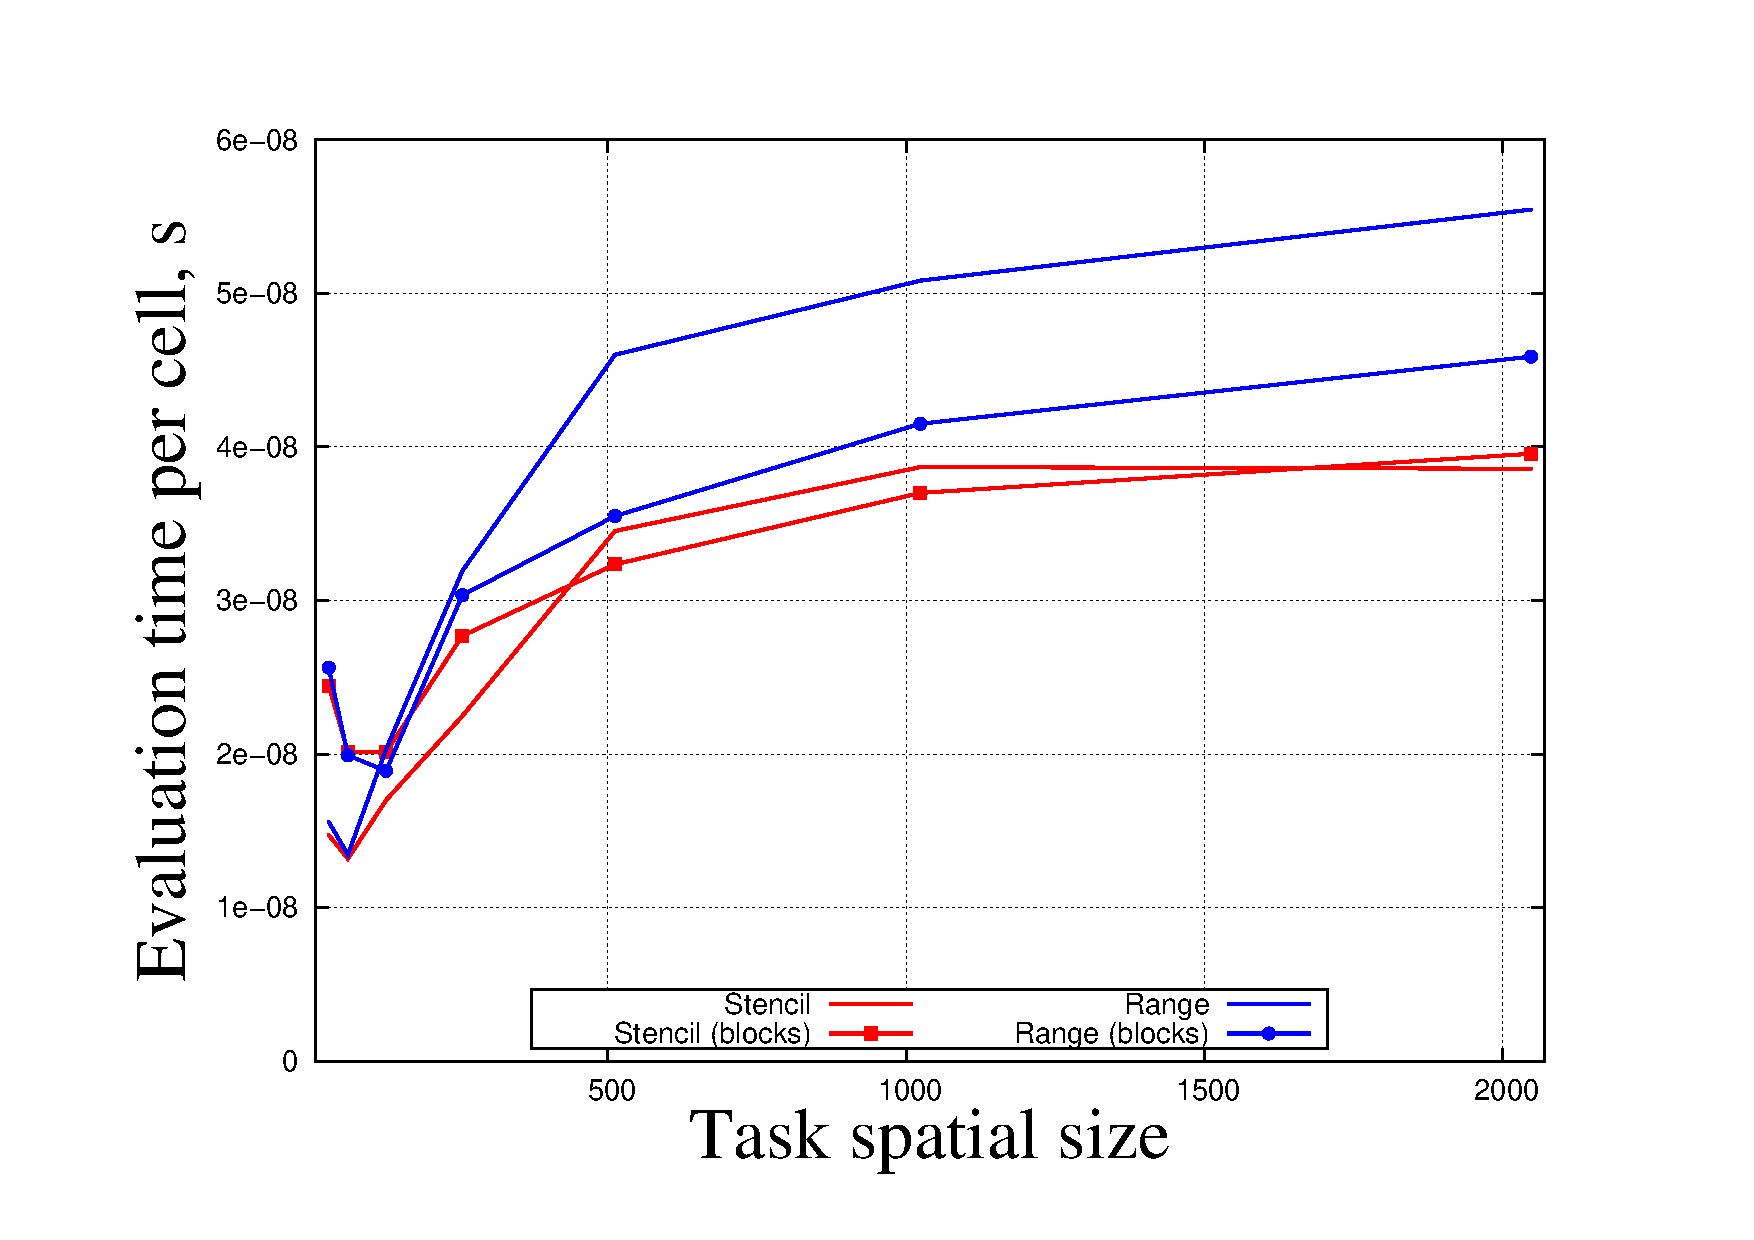
\includegraphics[width=1\textwidth]{2D_blocks_amd.pdf}}
\end{minipage}
\caption{Время выполнения 2D алгоритма с блоками для реализации на Blitz++
  в зависимости от пространственного размера задачи (AMD)}
\label{2D_blocks_amd}
\end{figure}
Как следует из графика, затраты на дополнительный код для реализации блоков дают
положительный выигрыш при размерах задачи от 256~x~256 элементов. Значительное
ускорение при такой реализации наблюдается лишь для операции $Range,$ а значит
реализация алгоритма метода FDTD при помощи этой операции с оптимально 
подобранным количеством блоков может служить полезной дополнительной опцией,
позволяющей быстрее обрабатывать задачи определённых размеров в 2D случае.
\newpage
\section{Сравнение быстродействия реализаций на разных
  платформах}
Все предыдущие результаты приведены для процессора $AMD Phenom II X4 965$ c 4 Гб
оперативной памяти. Для сравнения все указанные выши тесты были проверены
на $Intel Core I5$. Результаты представлены на графиках ниже.
\begin{figure}[h]
\begin{minipage}[h]{0.99\textwidth}
\center{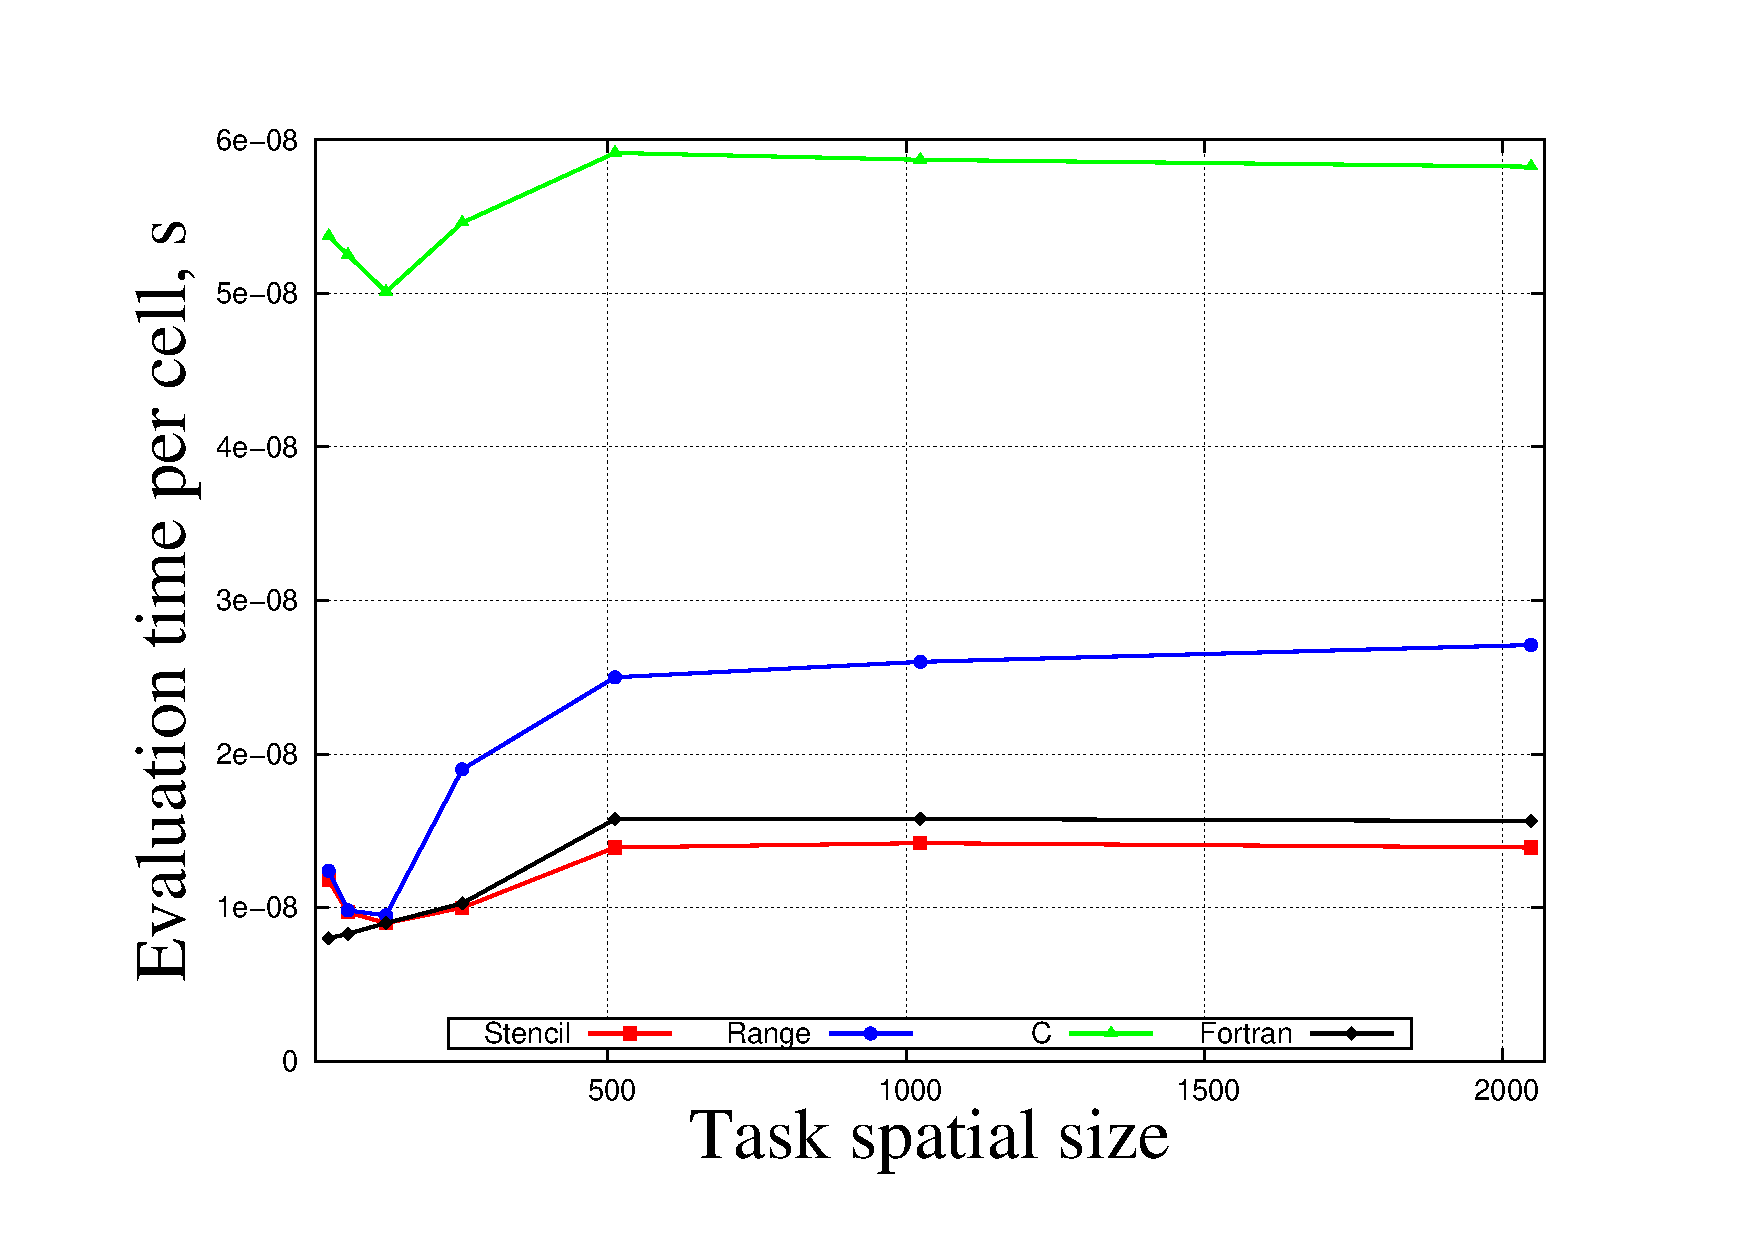
\includegraphics[width=0.7\textwidth]{2D_i5.pdf}}
\end{minipage}
\caption{Сравнение времён выполения 2D aлгоритма и в зависимости 
  от пространственного размера задачи для всех реализаций (i5)}
\label{2D_i5}
\end{figure}
\begin{figure}[h]
\begin{minipage}[h]{0.99\textwidth}
\center{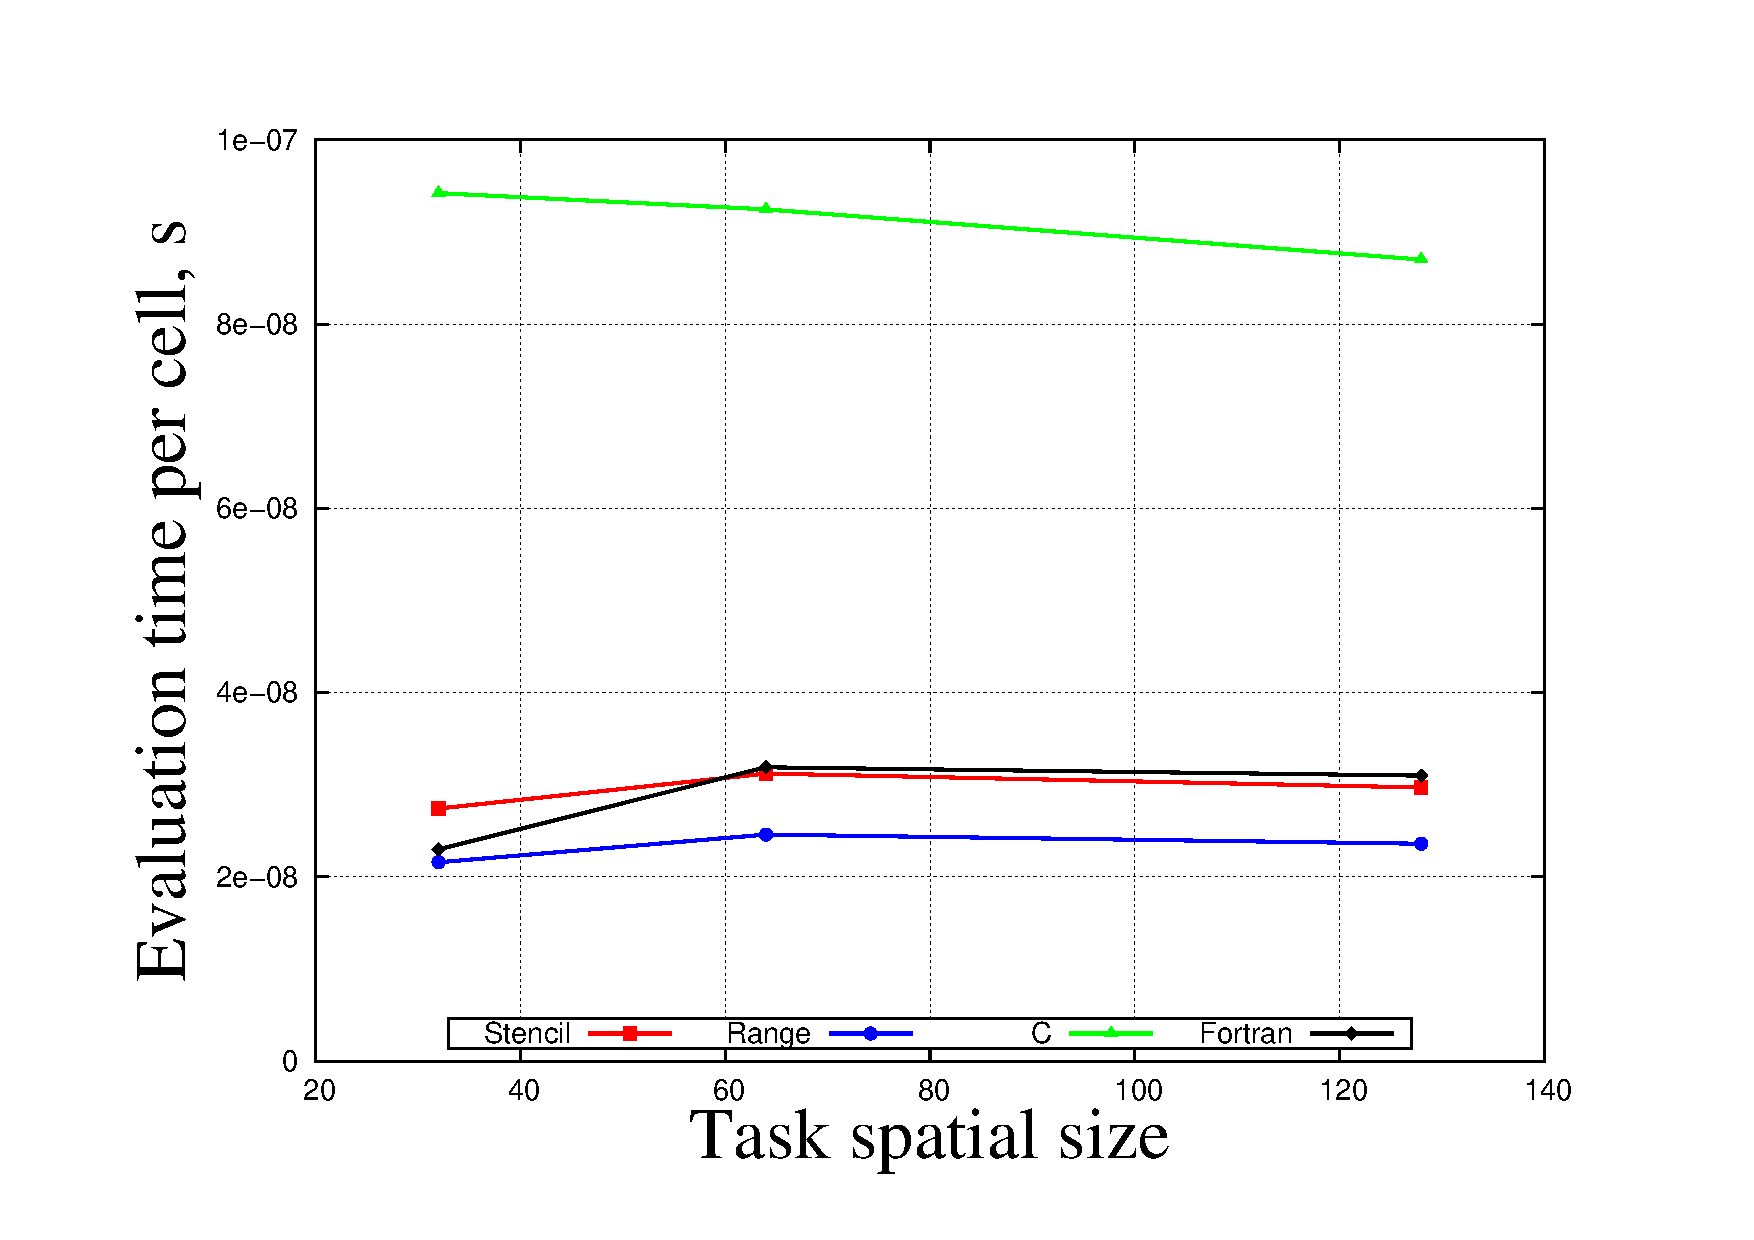
\includegraphics[width=0.7\textwidth]{3D_i5.pdf}}
\end{minipage}
\caption{Сравнение времён выполения 3D aлгоритма и в зависимости 
  от пространственного размера задачи для всех реализаций (i5)}
\label{3D_i5}
\end{figure}
\clearpage
\newpage
\begin{figure}[h]
\begin{minipage}[h]{1\textwidth}
\center{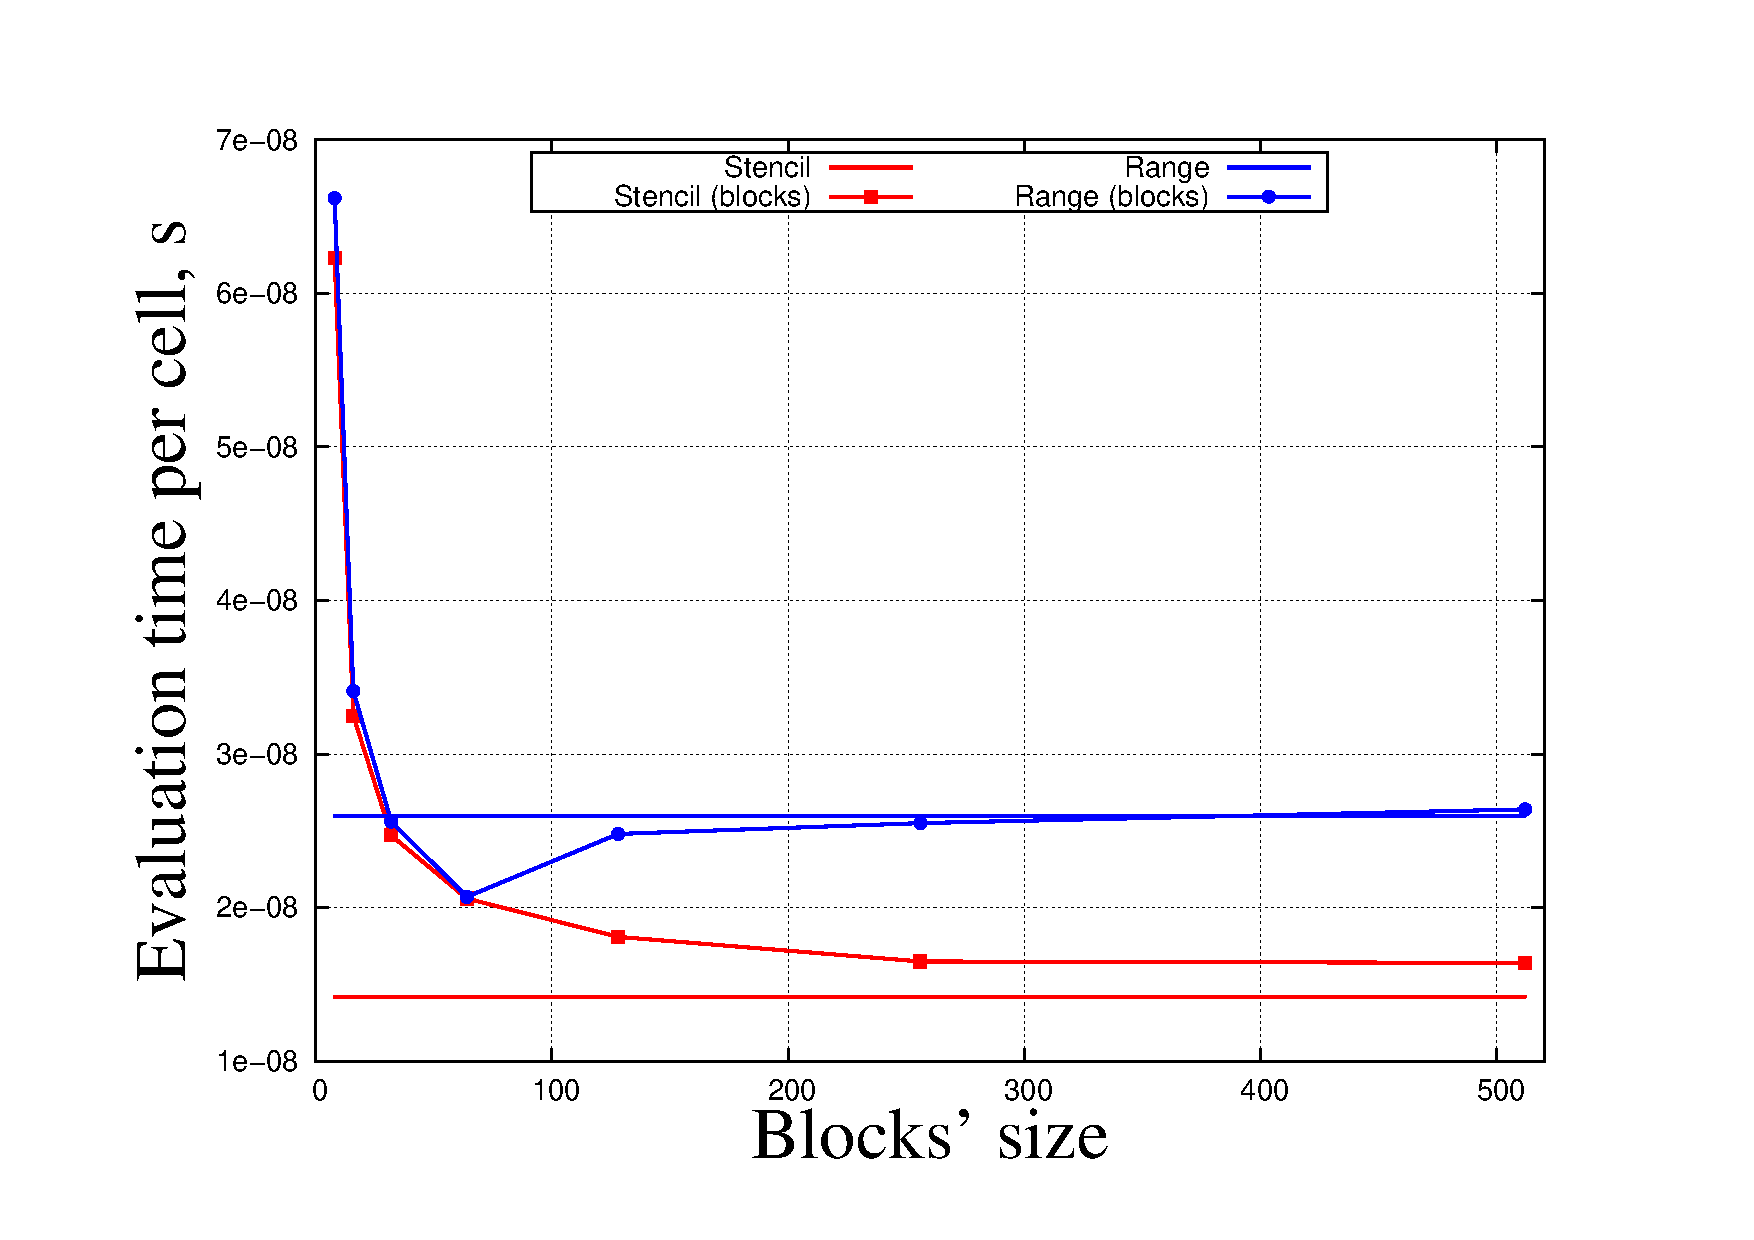
\includegraphics[width=0.65\textwidth]{1024_blocks_i5.pdf}}
\end{minipage}
\caption{Время выполнения 2D алгоритма с блоками для реализации на Blitz++ 
  для задачи 1024 x 1024 (i5)}
\label{1024_i5}
\end{figure}
\begin{figure}[h]
\begin{minipage}[h]{1\textwidth}
\center{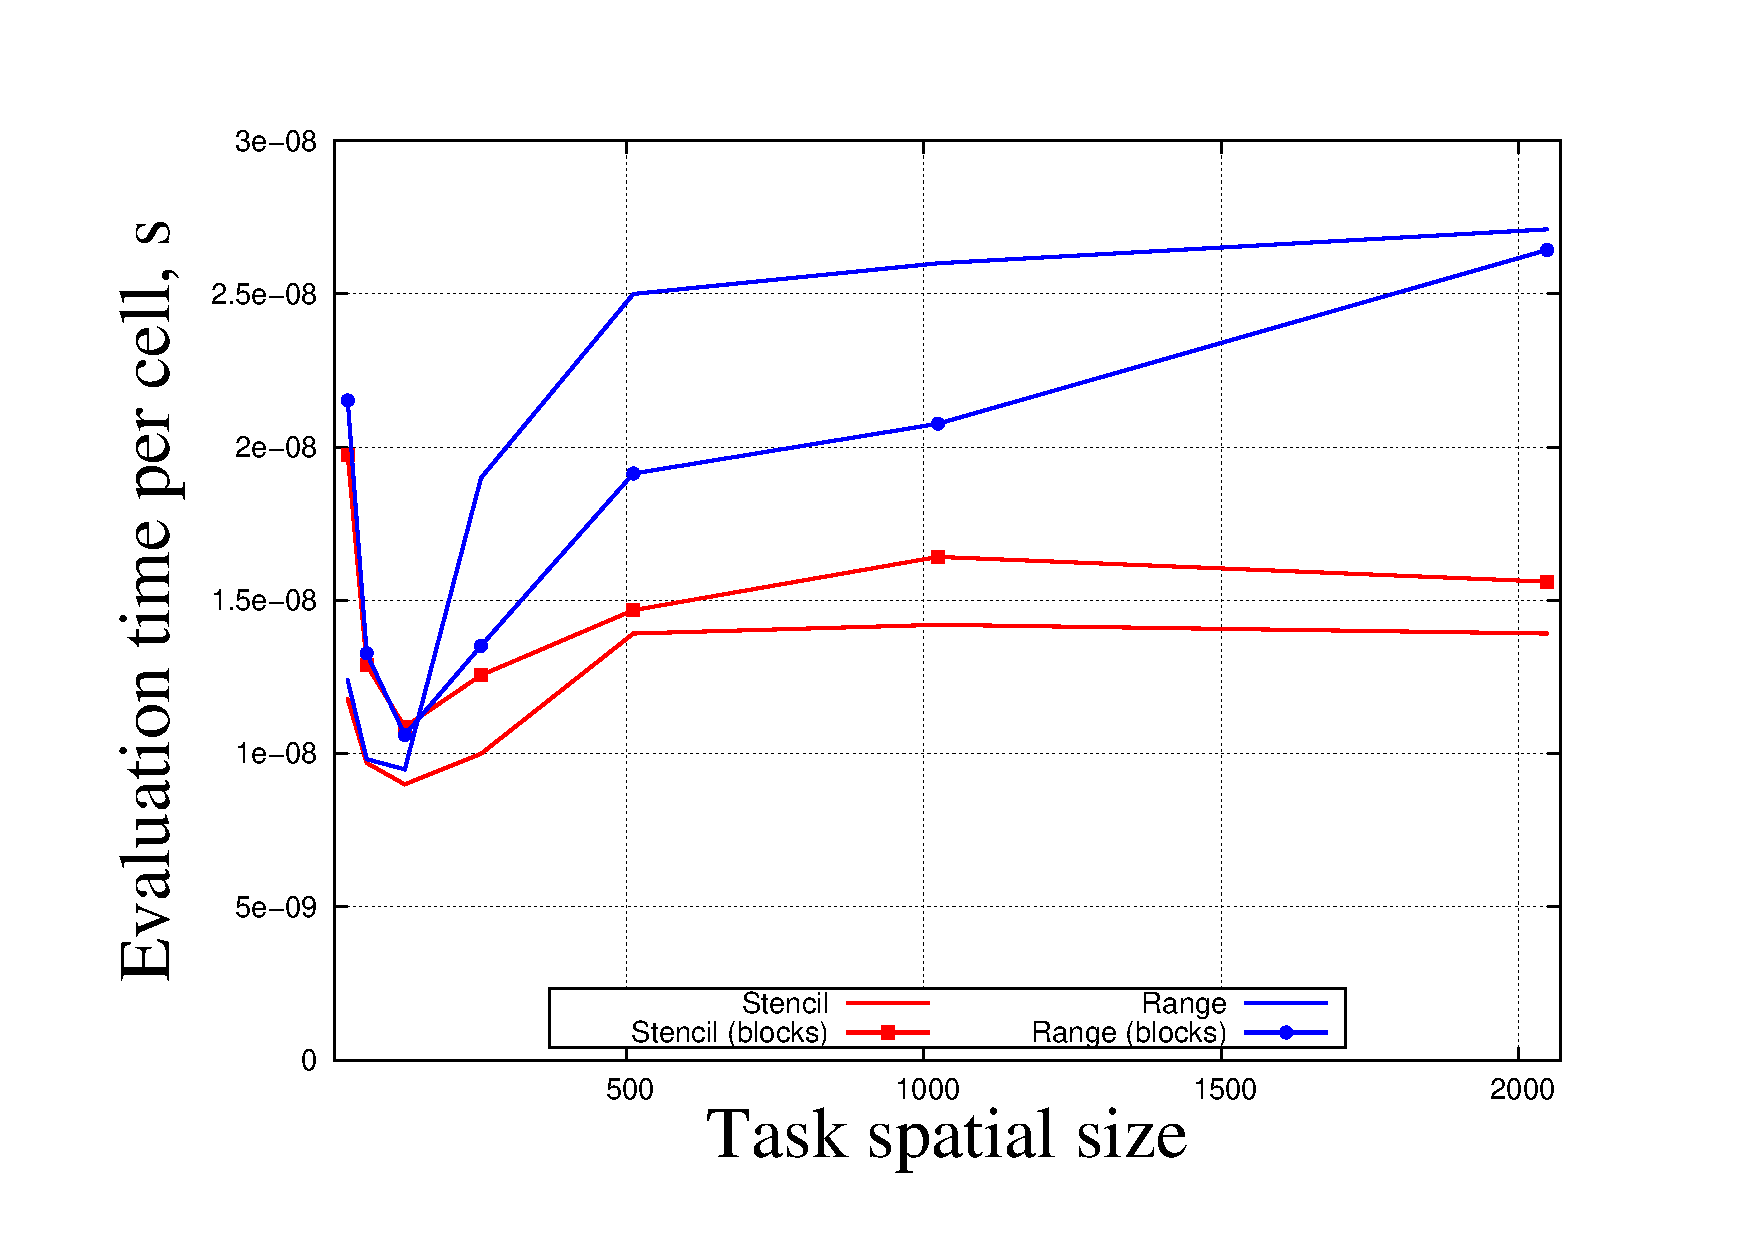
\includegraphics[width=0.65\textwidth]{2D_blocks_i5.pdf}}
\end{minipage}
\caption{Время выполнения 2D алгоритма с блоками для реализации на Blitz++
  в зависимости от пространственного размера задачи (i5)}
\label{2D_blocks_i5}
\end{figure}
\clearpage
\newpage
\section{Заключение}
C++ c использованием Blitz++ обладает сравнимой с Fortran'ом производительностью,
являясь при этом гораздо более выразительным языком, подходящим
для решения задач любого типа. Встроенные оптимизации библиотеки позволяют
получать высокопроизводительные программы практически без дополнительных
усилий со стороны пользователя. C++ вкупе с Blitz++ прекрасно подходят 
для реализации FDTD метода, обладая как необходимым быстродействием и 
простотой реализации алгоритмов, так и всеми стандартными средствами C++ 
для подготовки и обработки данных.
\renewcommand{\refname}{Список Литературы}
\begin{thebibliography}{10}
\bibitem{Yee1966}
  Kane Yee (1966). "Numerical solution of initial boundary value problems
  involving Maxwell's equations in isotropic media". Antennas and Propagation,
  IEEE Transactions on 14: 302–307. DOI:10.1109/TAP.1966.1138693
\bibitem{Taflove}
  Allen~Taflove,~Susan~C.~Hagness, Computational Electrodynamics: The Finite-
  Difference Time-Domain Method, Artech~House, INC.,~685~Canton~Street~Nordwood,
  MA,~02062
\bibitem{udfdtd}
  John~B.~Schneider, "Understanding the Finite-Difference Time-Domain Method"
\bibitem{Todd1997}
  Todd Veldhuizen, Scientific Computing: C++ versus Fortran
\bibitem{blitz_web}
  http://sourceforge.net/projects/blitz/
\end{thebibliography}
\end{document}
